%%% Template originaly created by Karol Kozioł (mail@karol-koziol.net) and modified for ShareLaTeX use

\documentclass[a4paper,11pt]{article}

\usepackage[T1]{fontenc}
\usepackage[spanish]{babel}
\usepackage[utf8]{inputenc}
\usepackage{graphicx}
\usepackage{xcolor}
\usepackage{wrapfig}

\renewcommand\familydefault{\sfdefault}
\usepackage{tgheros}
\usepackage[defaultmono]{droidmono}

\usepackage{amsmath,amssymb,amsthm,textcomp}
\usepackage{enumerate}
\usepackage{multicol}
\usepackage{tikz}

\usepackage{geometry}
\geometry{total={210mm,297mm},
left=25mm,right=25mm,%
bindingoffset=0mm, top=20mm,bottom=20mm}


\linespread{1.3}

\newcommand{\linia}{\rule{\linewidth}{0.5pt}}

% custom theorems if needed
\newtheoremstyle{mytheor}
    {1ex}{1ex}{\normalfont}{0pt}{\scshape}{.}{1ex}
    {{\thmname{#1 }}{\thmnumber{#2}}{\thmnote{ (#3)}}}

\theoremstyle{mytheor}
\newtheorem{defi}{Definition}

% my own titles
\makeatletter
\renewcommand{\maketitle}{
\begin{center}
\vspace{2ex}
{\huge \textsc{\@title}}
\vspace{1ex}
\\
\linia\\
\@author \hfill \@date
\vspace{4ex}
\end{center}
}
\makeatother
%%%

% custom footers and headers
\usepackage{fancyhdr}
\pagestyle{fancy}
\lhead{}
\chead{}
\rhead{}
\lfoot{Entrega \textnumero{}  2 - Proyecto Seguridad Informática}
\cfoot{}
\rfoot{Página \thepage}
\renewcommand{\headrulewidth}{0pt}
\renewcommand{\footrulewidth}{0pt}
%

% code listing settings
\usepackage{listings}
\lstset{
    language=Python,
    basicstyle=\footnotesize,
    frame=.2,
  xleftmargin=.2\textwidth, xrightmargin=.2\textwidth,
    basicstyle=\ttfamily\small,
    columns=fixed,
    extendedchars=true,
    breaklines=true,
    tabsize=6,
    prebreak=\raisebox{1ex}[1ex][1ex]{\ensuremath{\hookleftarrow}},
    showspaces=false,
    showstringspaces=false,
    keywordstyle=\color[rgb]{0.627,0.126,0.941},
    commentstyle=\color[rgb]{0.133,0.545,0.133},
    stringstyle=\color[rgb]{01,0,0},
    captionpos=t,
    escapeinside={\%*}{*)}
}

%%%----------%%%----------%%%----------%%%----------%%%

\begin{document}

\begin{titlepage} % Suppresses displaying the page number on the title page and the subsequent page counts as page 1
	
	\raggedleft % Right align the title page
	
	\rule{1pt}{\textheight} % Vertical line
	\hspace{0.05\textwidth} % Whitespace between the vertical line and title page text
	\parbox[b]{0.75\textwidth}{ % Paragraph box for holding the title page text, adjust the width to move the title page left or right on the page
	 \begin{tabularx}{\linewidth}{}
    \makecell{
\includegraphics[height=2cm]{logo}}
     \end{tabularx}
     \bigskip
     \vfill
		{\Huge\bfseries Entrega \textnumero{} 2 Proyecto\\[0.5\baselineskip] Seguridad ~ Informática}\\[2\baselineskip] % Title
		{\large\textsc{Auditoria de la Aplicación y}}\\
		{\large\textsc{Decompilación }}\\[1\baselineskip] % Subtitle or further description
		{\normalsize\textit{Camilo Zepeda Hoffmann}} % Author name, lower case for consistent small caps
		
		\vspace{0.5\textheight} % Whitespace between the title block and the publisher
		
		{\noindent Profesor~ Maximiliano~Vega\plogo}\\[\baselineskip] % Publisher and logo
		{\normalsize\textit{12 de Octubre 2017}}
	}

\end{titlepage}


\section{Resumen}

Ya en conocimiento de la relevancia y puntos importantes de lo que implica realizar una auditoría en todo tipo de sistema, se sostiene la misma ideología basada en la decompilación y comprobación respectiva a la seguridad de la aplicación escogida. 
En este caso al tratarse de Instagram; sistema que actualmente es delegado por el equipo de Facebook, se considera generar pruebas asociadas a las debilidades, exploits, fallas o no de la aplicación. Es por ésta razón que se propone dar a conocer los pasos efectuados para la visualización de los componentes asociados en conjunto con herramientas que faciliten la depuración de la aplicación, dejando así, la propuesta correspondiente a los futuros incrementales.

\section{Data Histórica de Vulnerabilidades}

A continuación se da a conocer un compilado de problemas relacionados al software y plataforma de Instagram, luego de la compra de la misma. Ahora bien, se considera éste periodo como relevante al ser las exposiciones más importante y connotadas de filtración de datos. 

\subsection{Vulnerabilidad en OAuth 2013}


\begin{wrapfigure}{r}{0.43\textwidth} 
\vspace{1pt}
  \begin{center}
    
\includegraphics[width=0.36\textwidth]{oauth}
    \label{fig:databaseUserTable}
  \end{center}
  \vspace{1pt}
\end{wrapfigure} 

Tras la compra de la Plataforma el año 2012 por Facebook, se logró encontrar fallas relacionadas a la privacidad, confidencialidad y filtración de datos, comprometiendo a los usuarios del software al existir errores del software ligados al protocolo OAuth, el cuál, realiza el control de autorización a terceros para acceder a la información, dando permisos bajo el servidor y un determinado cliente. Dicho problema abrió paso a problemas como el acceso a la lista de amigos en Facebook o filtración de imágenes $^{[1]}$.


\subsection{Cuentas Compartidas 2016}

\begin{wrapfigure}{l}{0.43\textwidth} 
\vspace{1pt}
  \begin{center}
    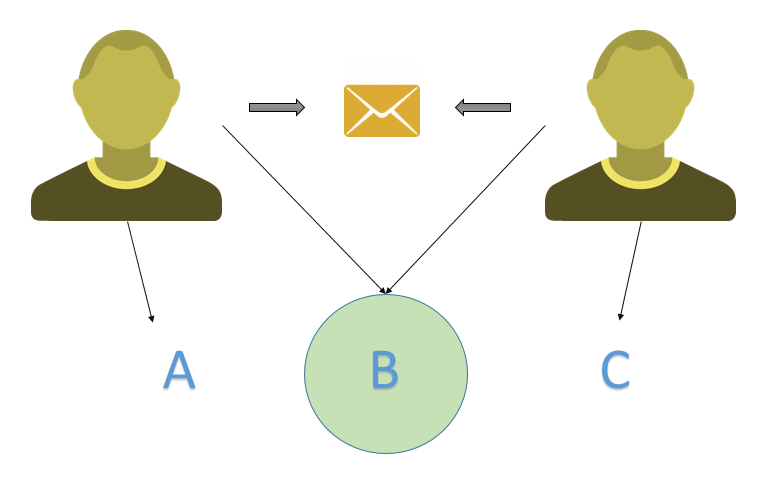
\includegraphics[width=0.4\textwidth]{compartidaig.png}
    \label{fig:databaseUserTable}
  \end{center}
  \vspace{2pt}
\end{wrapfigure} 

Problema relacionado al software en Sistema Android encontrado el 2016, el cual tiene como repercusión la vista de información no necesariamente del propietario, lo que implica un error en cuánto a la privacidad y confidencialidad de los datos. Entonces ésta vulnerabilidad consiste en la compartición de cuentas por parte de un Sujeto 1 v's un Sujeto 2, donde ambos ya sea por motivos de asociación u otros poseen una cuenta en común B, dando paso a la notificación de cuentas fuera de su alcance, ya que si por su parte el Sujeto 1 es propietario de la cuenta A y el Sujeto 2 es dueño de la cuenta B, se logra ver información desde A en C, aún sin ser propietario o usuario principal de ella $^{[2]}$. Por tanto, se implica una filtración de información fuera del consentimiento de cada sujeto.


\subsection{Hackeo de Cuentas 2017}


\begin{wrapfigure}{r}{0.43\textwidth} 
\vspace{2pt}
  \begin{center}
    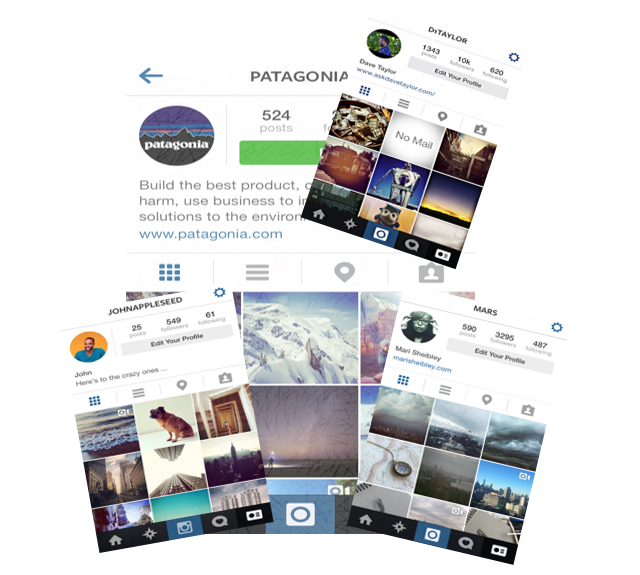
\includegraphics[width=0.45\textwidth]{accounts.png}
    \label{fig:databaseUserTable}
  \end{center}
  \vspace{2pt}
\end{wrapfigure} 

\bigskip

Actualmente la plataforma cuenta con un gran número de métodos y propiedades que mitigan las vulnerabilidades, aún bajo ésta tesis existen filtraciones de datos basados en ingeniería social o posibles errores de la plataforma, lo que el pasado mes de agosto del presente año se hizo de gran popularidad, logrando un hackeo masivo de cuentas, comprometiendo la seguridad de los usuarios en redes sociales. Llegando a circular datos de acceso a los perfiles de hasta \$10 dolares cada cuenta. La información fue almacenada en la base de datos \textbf{Doxagram} $^{[3]}$ en donde se realiza la venta y comercialización de la información.


\section{Análisis de la Aplicación}
Previo a la obtención y análisis de la aplicación dado los datos a obtener se propone definir los requerimientos base que conforman la actividad realizada. El listado de Herramientas utilizadas es:

\begin{itemize}
    \item \textbf{Página de Descarga}: se utiliza una página que disponga de la app.
    \item \textbf{Lionsec}: dado que es necesario decompilar la aplicación, se utiliza el nombrado sistema operativo, debido a sus multiples funciones y herramientas que faciliten el trabajo.
    \item \textbf{Apktool}: herramienta que realiza la lectura y depuración de la aplicación.
    \item \textbf{Dex2jar}: herramienta utilizada para convertir los diferentes .dex propios de android a .jar.
    \item \textbf{Java Decompiler}: utilizado para lograr depurar los archivos .jar.
\end{itemize}

\subsection{Obtención de la Aplicación}
En primera instancia es necesario conocer que la aplicación se encuentra disponible tanto para sistemas operativos iOs como Android, donde si bien es posible descargar ambos formatos no es posible decompilar los dos por igual. Cabe aclarar que se refiere a decompilar, como la obtención de toda la data proveniente de la aplicación. Entonces si bien, iOs dispone de los layouts o vistas, las cuales pueden ser editadas no se logra editar y ver los códigos base de la app. 

\begin{wrapfigure}{l}{0.5\textwidth} 
\vspace{2pt}
  \begin{center}
    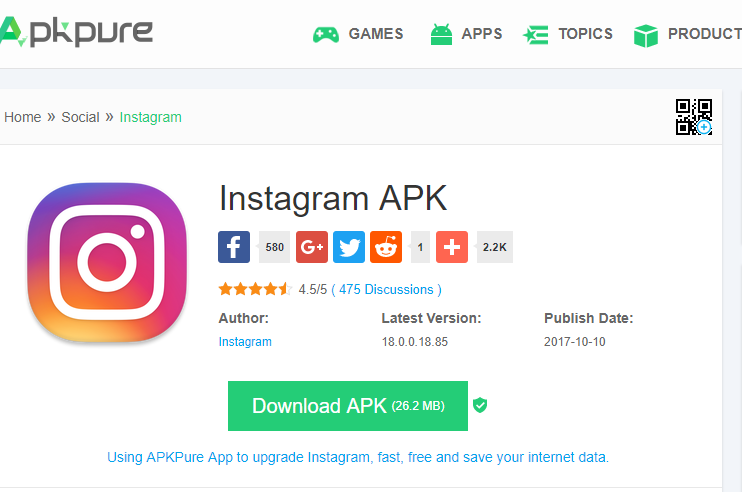
\includegraphics[width=0.45\textwidth]{apkpure.png}
    \label{fig:databaseUserTable}
  \end{center}
  \vspace{1pt}
\end{wrapfigure} 
Entonces en concordancia con lo anterior, se realiza un análisis de la aplicación \textbf{.apk} (Sistema Operativo Android) al ser más amigable al momento de depurar, entregando una serie de archivos y datos correspondientes a la plataforma. Para lograr la obtención de la aplicación se hace uso de \textbf{ApkPure} página que dispone de la última versión de Instagram descargable para el computador. 
Ya en obtención de la aplicación y bajo el uso de las herramientas mencionadas anteriormente se procede a la depuración de la app.\\



\subsection{Decompilación de la Aplicación}
Con tal de lograr un mejor entendimiento de lo realizado se describe una serie de pasos de la mano con el material obtenido, en formato de imagen o similar.


\begin{itemize}
    \item \textbf{Paso 1}: ya en posesión de la .apk correspondiente a la aplicación la primera actividad fue el transformar el archivo de:
    
    \begin{verbatim}
        Intagram.apk => Instagram.zip
    \end{verbatim}
    
    \begin{figure}[!h]
    \centering
    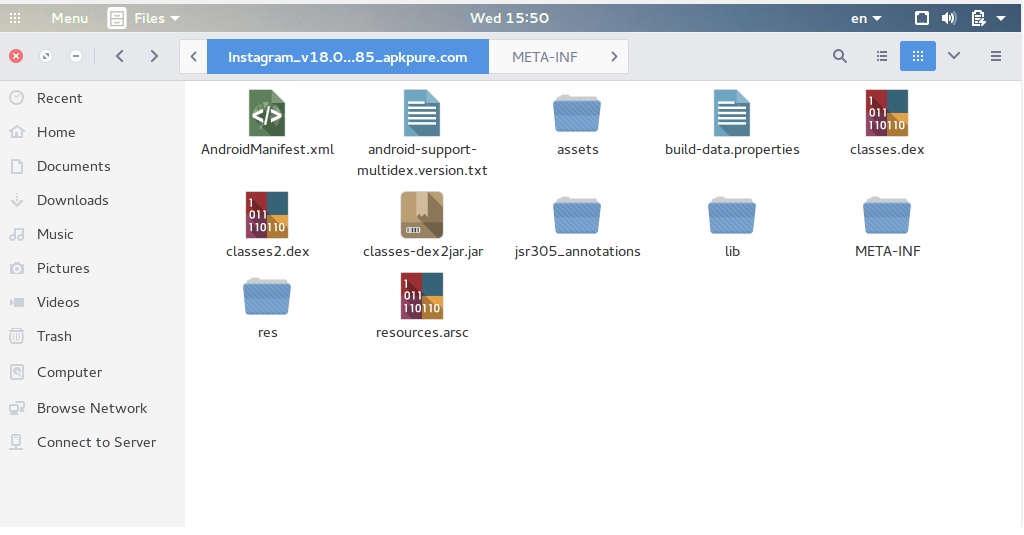
\includegraphics[scale=0.5]{decompiladaapk.png}
    \label{fig:my_label}
    \end{figure}
    
    De la conversión anterior se obtiene acceso a los archivos en bruto de la aplicación, así no, no es posible observar los xml, java o react de la misma, ya que aún no se ha depurado a cabalidad. Igualmente, se obtienen los \textbf{.dex} equivalente a las clases utilizadas por la app. 
        
    
    \item \textbf{Paso 2}: ya extraídos los archivos anteriormente mencionados, se puede observar la carpeta \textbf{META-INF} equivalente al certificado de los desarrolladores de la aplicación, la cual al revisar los datos internos se determina que  se usa Hashing Sha1 para el certificado de desarrollador y cifrado RSA, para el certificado entregado por Android. Lo dicho puede verse en la siguiente figura:
    
     \begin{figure}[!h]
    \centering
    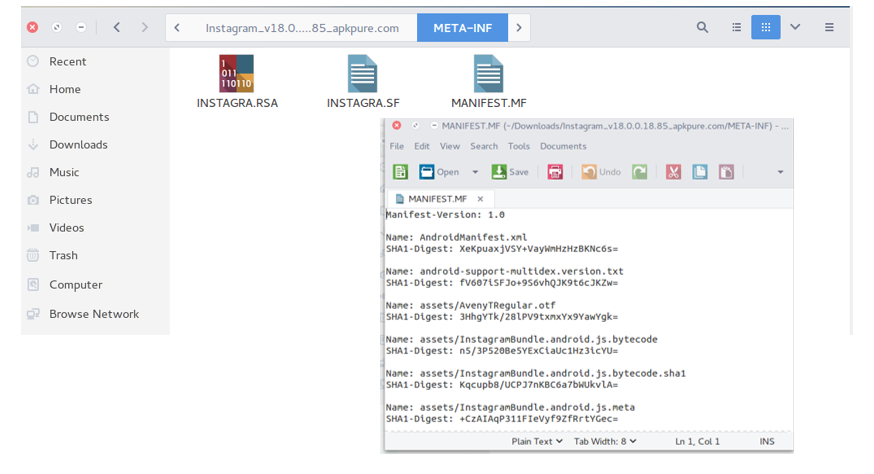
\includegraphics[scale=0.5]{meta-inf2.png}
    \label{fig:my_label}
    \end{figure}
    
    
    \item \textbf{Paso 3}: Una vez realizado los pasos anteriores fue posible determinar que no se pueden ver tanto los xml, como los java provenientes de la aplicación. Es por esta razón que se hace uso de software \textbf{ApkTool} ya interno en Lionsec.
    Ya familiarizado con la herramienta se realiza el siguiente comando:
    
    \begin{verbatim}
        apktool d Intagram.apk
    \end{verbatim}  
    
    Donde se define \textbf{d} como la lectura del archivo, obteniendo entonces los siguientes archivos:
    
       \begin{figure}[!h]
    \centering
    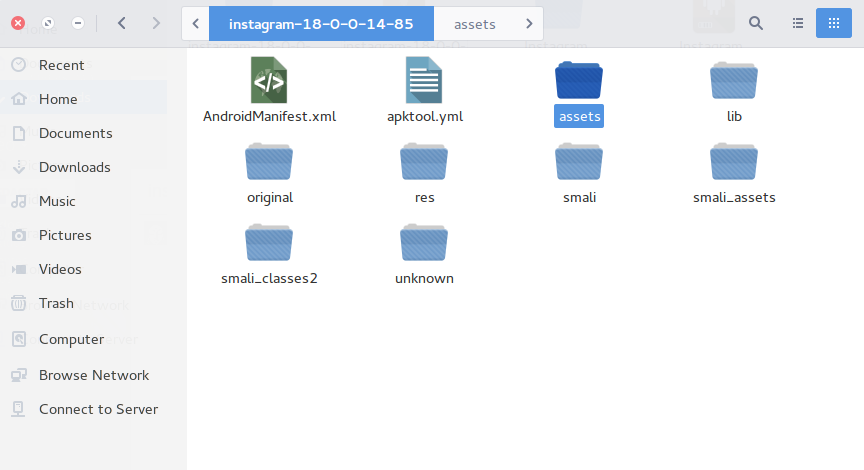
\includegraphics[scale=0.5]{apktool.png}
    \label{fig:my_label}
    \end{figure}
    
    
    
    \item \textbf{Paso 4}: Finalmente tras disponer de la información y datos pertinentes a la depuración de la aplicación. Es necesario revisar los datos obtenidos e información relevante.
    Los primeros datos revisados fueron los XmlAndroid, los cuales definen  parte de los requerimientos y facultades que asocia la aplicación para su desempeño. La siguiente figura da una perspectiva de lo visto.
    
     \begin{figure}[!h]
    \centering
    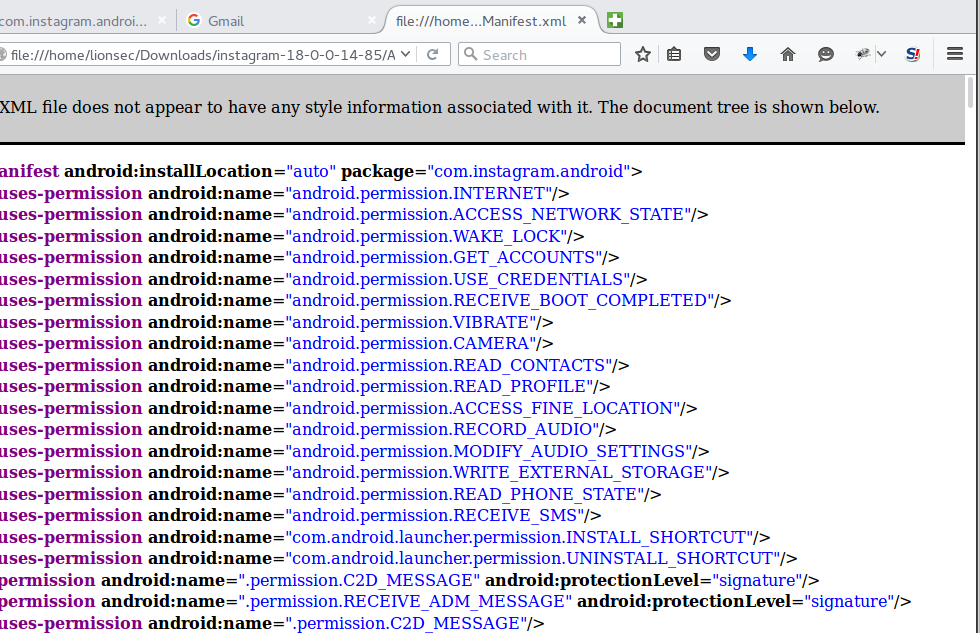
\includegraphics[scale=0.5]{xml.png}
    \label{fig:my_label}
    \end{figure}
    
    Si bien se puede encontrar una serie de disposiciones y permisos relacionados a la aplicación, no se considera un punto relevante para la depuración, ya que son puntos relativamente comunes para la aplicación, dígase, no se encuentra anomalías que puedan ser explotables en futuros incrementales.\\
    
    Por otra parte, mediante el uso de la herramienta dex2jar, se realiza una conversión de las clases intrinsecas en la aplicación, mediante el comando:
    
    \begin{verbatim}
        d2j-dex2jar classes.dex
    \end{verbatim}
    
        
     \begin{figure}[!h]
    \centering
    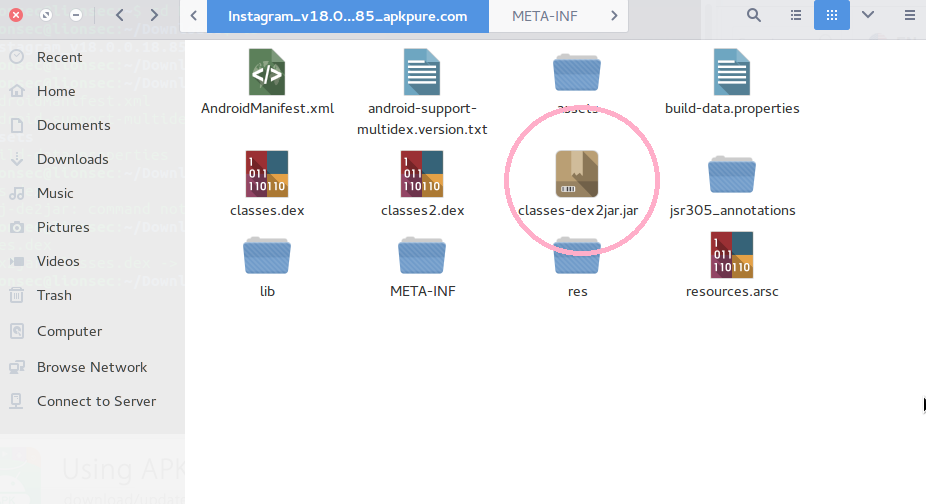
\includegraphics[scale=0.5]{jarclases.png}
    \label{fig:my_label}
    \end{figure}
    
    
    Lo que convierte los archivos a un formato .jar, el que por medio de una Java Decompiler y jd-gui interno del mismo, puede lograrse un análisis de los archivos java desarrollados en la aplicación.\\
    
    Por último se realiza una revisión de los archivos React, los cuales se encuentran en formato \textbf{.smali} propio de Java. Obteniendo entonces lo siguiente:
    
           
     \begin{figure}[!h]
    \centering
    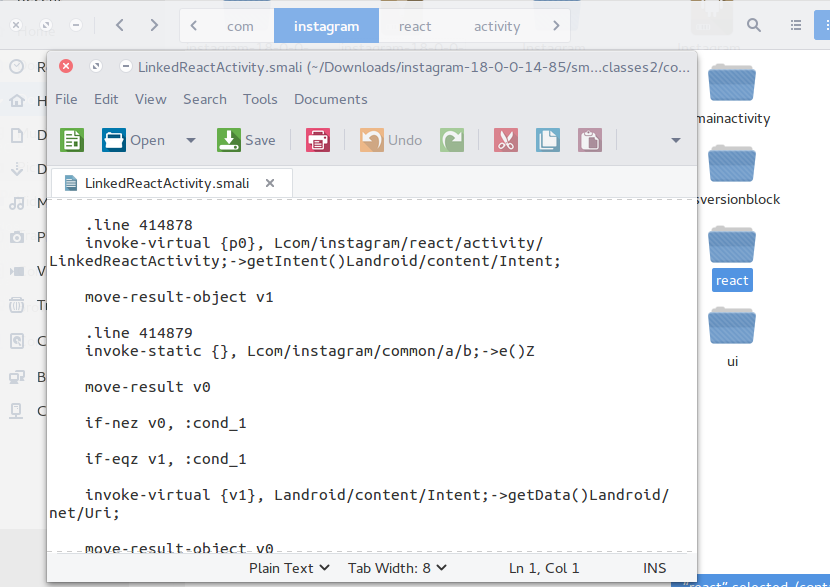
\includegraphics[scale=0.5]{react.png}
    \label{fig:my_label}
    \end{figure}
    
    Cabe destacar que los archivos vistos en la figura anterior tienen una real validez en cuanto a vulnerabilidades explotables para la auditoría a realizar, ya que dichas opciones son las actividades, acciones y funciones propias de la aplicación, dando apertura a protocolos, urls, traspaso de información y otras actividades que compromenten la aplicación.
    
    
    
\end{itemize}


\subsection{Propuestas para Tercer Incremento}

Con el fin de lograr una mayor comprensión de lo propuesto se define el siguiente listado.

\begin{itemize}
    \item Analizar en profundidad las funciones Internas React, depurando la información.
    \item Buscar vulnerabilidades correspondientes a la página de Instagram (inyecciones SQL).
    \item Buscar posibles Scripts utilizados para robar información.
    \item Analizar Servicios utilizados por la aplicación.
    \item Depurar en profundidad los archivos pertinentes de la app.
    \item Instalar la aplicación, con tal de analizar la BD interna generada por la misma.
\end{itemize}



\newpage










\begin{thebibliography}{1}
\bibitem{Oauth}
A. Plaza, "Un fallo de seguridad en Instagram muestra la vulnerabilidad de las cuentas | Hipertextual", Hipertextual, 2017. [Online]. Available: \url{https://hipertextual.com/2013/05/fallo-de-seguridad-en-instagram}. [Accessed: 11- Oct- 2017].


\bibitem{cuentas}
"La posibilidad de usar varias cuentas en Instagram presenta un fallo de seguridad - TreceBits", TreceBits, 2017. [Online]. Available: \url{http://www.trecebits.com/2016/02/16/la-posibilidad-de-usar-varias-cuentas-en-instagram-presenta-un-fallo-de-seguridad/}. [Accessed: 11- Oct- 2017].

\bibitem{hack}
"El hackeo a Instagram, más grave de lo esperado: 6 millones de cuentas", ADSLZone, 2017. [Online]. Available: \url{https://www.adslzone.net/2017/09/02/el-hackeo-instagram-mas-grave-de-lo-esperado-6-millones-de-cuentas/}. [Accessed: 11- Oct- 2017].

\bibitem{appirater}
https://www.buzztouch.com/forum/thread.php?tid=B60C6EE41CD7D289048B0F4

\bibitem{appirater2}
https://github.com/arashpayan/appirater

\bibitem{reachability}
https://iphoneros.com/44273/asi-es-el-modo-reachability-para-poder-utilizar-el-iphone-6-plus-con-una-sola-mano-video

\bibitem{curl}
https://curl.haxx.se/docs/history.html

\end{thebibliography}

\newpage



\end{document}
